\documentclass[crop,tikz]{standalone}
\usepackage{tkz-base}
\usepackage{pgfplots}
\usetikzlibrary {shapes.multipart}

\pgfplotsset{compat=1.18}
 \begin{document} 

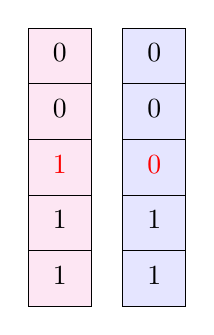
\begin{tikzpicture}[node distance = 0pt,
    VMPN/.style = {rectangle split,rectangle split parts=5,
                    draw,
                    fill=#1,
                    text width=0.8cm, align=center,
                    inner sep=0pt, outer sep=0pt}
                            ]

    \tikzset{every node/.style={rectangle split, draw}}
    
    % \node[rectangle split part fill={magenta!30}]  {};
    % \node[rectangle split part fill={green!50}, opacity = 0]at()  {};
    % \node[rectangle split part fill={blue!30}] {};
    \node (n1)  [VMPN=magenta!10]  {\nodepart{one} ~\\ 0\\[-1ex]~
                        \nodepart{two} ~\\ 0\\[-1ex]~
                        \nodepart{three} ~\\ {\color{red} 1}\\[-1ex]~
                        \nodepart{four} ~\\ 1\\[-1ex]~
                        \nodepart{five} ~\\ 1\\[-1ex]~
                        };
    \node (n2) [right=of n1, opacity = 0] {};
    \node (n3)  [VMPN=blue!10,
            right=of n2]  {\nodepart{one} ~\\ 0\\[-1ex]~
                        \nodepart{two} ~\\ 0\\[-1ex]~
                        \nodepart{three} ~\\\color{red} 0\\[-1ex]~
                        \nodepart{four} ~\\ 1\\[-1ex]~
                        \nodepart{five} ~\\ 1\\[-1ex]~
                        };
\end{tikzpicture}

\end{document} 